%rubber: module pdflatex
\documentclass[11pt,a4paper]{article}
\usepackage{microtype}\usepackage{mathptmx}
\usepackage{sdp_doc} % SDP style file
\usepackage[english]{babel} 
\usepackage{listings}
\usepackage{hyperref}

\usepackage{amsthm}
\usepackage{thmtools}
\usepackage[dvipsnames]{xcolor}
\usepackage{algpseudocode}

\declaretheoremstyle[spaceabove=6pt, spacebelow=6pt,
headfont=\normalfont\bfseries,
notefont=\mdseries, notebraces={(}{)},
bodyfont=\normalfont,
postheadspace=1em,
headpunct=\\,
notebraces=\ \ ,
qed=]{ExampleStyle}
\declaretheorem[style=ExampleStyle,shaded={rulecolor=Lavender,
rulewidth=1pt, margin=10pt, bgcolor={rgb}{0.98,0.98,1}}]{Example}




\definecolor{antiquewhite}{rgb}{0.98, 0.92, 0.86}

\lstset{ %
  backgroundcolor=\color{antiquewhite},   % choose the background color; you must add \usepackage{color} or \usepackage{xcolor}
  basicstyle=\footnotesize,        % the size of the fonts that are used for the code
  captionpos=b,                    % sets the caption-position to bottom
  frame=single}


%%%%%%%%% START OF USER SETTINGS %%%%%%%%%%%%%%%%%%

% Enter here some information needed to fill in the template Title to appear
% on the front pages (will be filled in via the \sdpfrontpage command)
\newcommand{\bigdoctitle}{SDP Dataflow Environment\xspace}
% Title to go in the "Document Status Sheet" Document number
\newcommand{\docnr}{RP\_A0999\xspace}
% Context
\newcommand{\context}{(SDP Work Package)}
% Revision
\newcommand{\revision}{0.92\xspace}
% Author(s)
\newcommand{\docauthor}{B.\ Nikolic, P.\ Braam\xspace}
% Lead author (goes in the footer)
\newcommand{\leadauthor}{B.\ Nikolic\xspace}
% Release
\newcommand{\release}{1.0\xspace}
% Date of the document release, format: Month YYYY (e.g., August 2008)
\newcommand{\docudate}{2015-02-09\xspace}
% Document classification
\newcommand{\classification}{Unrestricted}
% Status of the document (draft/final/etc.)
\newcommand{\docstatus}{Draft\xspace}


% Table with signatures
\newcommand{\signaturetable}{
  \begin{tabularx}{\textwidth}{|X|X|X|}
      \hline
      Name & Designation & Affilitation\\
      \hline
      B. Nikolic& Lead Author& University of Cambridge \\
      \hline
      Signature \& Date: & & \\
      & & \\
      & & \\
      \hline
      Name & Designation & Affilitation\\
      \hline
      & & \\
      \hline
      Signature \& Date: & & \\
      & & \\
      & & \\
      \hline
  \end{tabularx}
}

  % Table with version numbers
  \newcommand{\versiontable}{
  \begin{tabularx}{\textwidth}{|X|X|X|X|}
        \hline
        \bf{Version} & {\bf Date of issue} & {\bf Prepared by} & {\bf Comments}\\
        \hline
        1.0 & & & \\
        \hline
      \end{tabularx}
  }

% Table with affiliations
\newcommand{\organisationtable}{
\begin{center}
 \sffamily{\bf ORGANISATION DETAILS}\end{center}
    \begin{table}[htbp]
      \centering
      \begin{tabular}[htbp]{|l|l|}
        \hline
        Name & Science Data Processor Consortium\\
        \hline
      \end{tabular}
    \end{table}
  }

%%%%%%%%%%%%% END OF USER SETTINGS %%%%%%%%%%%%%%%%%%%



\begin{document}

% load automatic pages
\sdpfrontpage

\sdptableofcontents

% Add here the abbreviations used in your document
\sdplistofabbreviations
\begin{basedescript}{\desclabelstyle{\pushlabel}\desclabelwidth{6em}}
    \item[SOMETHING] Something \vspace{-0.2cm}
    \item[OTHER] Other something \vspace{-0.2cm}
    \item[OTHER] Other other something \vspace{-0.2cm}
\end{basedescript} 

% Add here the symbols used in your document
\sdplistofsymbols
\begin{basedescript}{\desclabelstyle{\pushlabel}\desclabelwidth{6em}}
    \item[$N_\mathrm{something}$] Number of somethings \vspace{-0.2cm}
    \item[OTHER] Other something \vspace{-0.2cm}
    \item[OTHER] Other other something \vspace{-0.2cm}
\end{basedescript} 


\sdplistoffigures

\sdplistoftables

% Add here the executive summary
\sdpsummary

The purpose of this document is to familiarise the reader with the
dataflow programming model and describe why this model is likely to
satisfy the requirements of the Science Data Processor. We then
describe concepts that accompany a data flow system, and the
relationship between the SDP systems architecture and the data flow
system.  Coverage of these four topics makes up the central sections
of this document.  A glossary at the end of this defines terminology.
The remainder of the introduction tries to describe at what level of
detail the current exposition proceeds.

% Add to the table the list of applicable and reference documents
% (this is NOT meant for your usual bibiliography, only for SKA docs)
\sdpreferencedocs

\subsection*{Applicable Documents}

The following documents are applicable to the extent stated herein. In the
event of conflict between the contents of the applicable documents and this
document, \emph{the applicable documents} shall take precedence.

\begin{center}{
\begin{tabularx}{\textwidth}{|X|X|}
    \hline
    \bf{Reference} & \bf{Reference}\\
    \bf{Number} & \\
    \hline
\end{tabularx}}
\end{center}

\subsection*{Reference Documents}

The following documents are referenced in this document. In the event of
conflict between the contents of the referenced documents and this document,
\emph{this document} shall take precedence.

\begin{center}{
\begin{tabularx}{\textwidth}{|X|X|}
    \hline
    \bf{Reference} & \bf{Reference}\\
    \bf{Number} & \\
    \hline
    RD01 & Science Data Processor Architecture\\\hline
    RD02 & Science Data Processor Pipelines Element Design Report\\\hline
    RD03 & COMP Element Design Report
  \end{tabularx}}
\end{center}



% The actual content goes here
\newpage
\section{Introduction}

We use the words dataflow {\bf program} for the domain specific
description of the computation that needs to done, e.g., the imaging
pipeline for a radio telescope.  We distinguish this from the dataflow
{\bf system}, which refers to a particular implementation enabling one
to write such programs. For example, a dataflow programming language
or a library with C-like API can both be dataflow systems.  We use the
words computing {\bf system architecture} to describe the hardware
environment on which the dataflow programs and the runtime of the
dataflow system can execute.  Finally, we use the words dataflow {\bf
  environment} to describe all of these components - the dataflow
programs, the dataflow system and the computing system architecture -
together to discuss for example the actual execution of programs on a
cluster of computers.

SDP will embed the dataflow system in the upper software layers of the
SDP system which will be executed on commodity hardware and making use
of more conventional software layers (this is further described in
Section~\ref{sec:sdp-syst-arch}). This is contrast to some past
dataflow systems that combined the dataflow model with specialised
dataflow hardware.

This document does neither recommend detailed choices of features or
particular choices of dataflow systems.  Instead, it is concerned with
an explanation of the high level application of data flow techniques
to SDP imaging, and requirements for dataflow systems that must or
should be met.

\section{Dataflow Programs}

\subsection{Concepts in dataflow programming}

\underline{Actors} are the basic units of computation in the dataflow
program. In very fine grained dataflow programs (e.g., GPU programs)
they can represent individual processor instructions but in the case
of SDP they will represent much larger units of computation, ranging
in size from a group of routines up to a ``task'' in a radio-astronomy
application such as CASA.  

Actors explicitly specify their input and output data which are
represented by \underline{data objects}. The data objects may be large
data structures such as arrays of numbers, or even data with a complex
models such as a radio astronomy Measurement Set. Data objects are the
units of data which are passed between actors through
\underline{channels} (which may transform the data). In the case of
the SDP the channels may range from a null operation where memory
containing the data object is simply handed over from one actor to
another, up to complex channels which buffer data on storage devices
or transmit it over the network.

A dataflow \underline{program} is specification of actors and how the
input of each is connected through a channel with the outputs of other
actors. In the case of SDP the dataflow programs will specify the
processing of input data through to the science-ready data
products. They replace the functionality of scripts and high-level
routines in packages like CASA and ASKAPSoft. The SDP dataflow
programs are further discussed in Section \ref{sec:ska-sdp-dataflow}.

The specification in the dataflow program is often called the
\underline{dataflow graph} or the data dependency graph: the actors
are the nodes of the graph and the channels are its edges. As we will
see momentarily, although such graph is a precise conceptual
representation of the dataflow program, dataflow programs are not
usually specified by explicitly instantiating such a graph, but rather
in a more conventional programming language mechanisms. In fact,
scalable dataflow
\citep{Bosilca6008964,Wozniak:2012:TDD:2443416.2443421} systems never
instantiate the full graph but traverse it symbolically and
instantiate explicitly only a small windows around which execution is
happening.

Computations in dataflow programs are not triggered by fetching
instructions sequentially (in fact, there is no single implicit
sequence of instructions in a dataflow program). Instead, computation
by the \underline{actors} is triggered by the readiness of
\underline{data objects} on the inputs of these actors. The arrival of
the entire object determines readiness: large objects are treated as
indivisible tokens.  The fact that a computation is triggered does not
mean it has to begin executing immediately upon the trigger: it could
be placed in set of ready to execute (“fireable”) actions and executed
some time later.

In {\bf demand-driven} dataflow programs the actions to execute from
the fireable set are determined by tracing back from the desired
outputs of the program to all intermediate actions that produce
intermediate data products, and so it is even possible that not all
triggered actions get executed. In {\bf data-driven} dataflow programs
all fireable actions are executed, usually using a queue system if not
immediately upon the trigger. The data-driven approach is well matched
to the objectives of the SDP since all of the data supplied to the SDP
are expected to be incorporated into the science-ready data products.


The structure of a dataflow program therefore specifies how initial
data is provided to the system and what happens when data flows
through actors to a final output.

Input nodes of the graph, i.e. nodes without input channels represent
input data for a dataflow program.  Upon program start, input nodes
start delivering data objects to their output channels and it is often
convenient to identify the input nodes with their output
channels. Input nodes may be triggered for delivery multiple
times\footnote{In case of the SDP the dimensions of the input data are
  determined by the scheduling block being observed and so are known
  in advance of the beginning of execution of the dataflow program.}.

Nodes in the graph without output channels represent results of the dataflow program.

There is a vast literature concerning dataflow programs of the kind
described above \citep[see the review
by][]{Johnston:2004:ADP:1013208.1013209}, and there are numerous
variations on the concepts and numerous detailed choices in these
concepts.  Some dataflow models have been described and studied in
mathematical detail, such as \cite{Hewitt:1973:UMA:1624775.1624804}
actor model, while other dataflow models are merely add-on libraries
to general purpose programming languages.

Similar variations exist in terms of typing the data that is
exchanged: it is sometimes precisely typed and in other systems merely
a buffer. Secondly we will just illustrate a few examples of alternate
choices in data flow systems:
\begin{enumerate}
  \item When describing the availability of data
  to trigger computation, must just one or all of multiple pieces of
  data be available to define readiness?  
\item Do the channels have a large or finite buffer space?
\end{enumerate}

\subsection{Concurrency model}
 
All actors and channels may compute concurrently but do not share any
data objects. The ownership of data objects, i.e. the locality of the
objects in the graph, is a central conceptual benefit\footnote{The
  converse of this is that there is a drawback in that the lack of
  shared data requires duplication of data when they are mutable and
  accessible from more than one actor. The impact of this can
  generally be reduced by having smaller tokens, i.e., data objects,
  passing on channels. Duplication of data in order to enable scalable
  parallelism is adopted in the SDP Architecture document as one of
  the necessary ways of enabling scalability.} of data flow computing
because the exclusive access to the data objects by defined elements
of the data flow graph introduces modularity. Indeed, the most common
problem in multithreading legacy imperative programs is identifying
concurrent data access.


\begin{Example}[A simple dataflow program]

A good example is a program that reads a vector and sums up the
 coordinates.  The input node reads the vector, hands this vector to
  an actor.  The actor is fired when the vector is e.g. in memory and
  then the actor adds the elements and writes the output.

illustration 1

The above example becomes more interesting if we instead partition the vector into N chunks. Now multiple – namely N - input nodes can read the chunks in parallel, and N actors can add the chunks coordinates in parallel and a collector can gather the partial sums and write the output.  

illustration 2

Conceptual pseudocode:
\begin{algorithmic}
  \State $a\gets \textrm{readFile "a"}$
  \State $b\gets \textrm{readFile "b"}$
  \State $c\gets  \textrm{+/} \quad a\times b$
\end{algorithmic}

In pseudo code, a dataflow program doing precisely this can be written as:
\begin{lstlisting}
master_actor (fileName, CAD)
    fork(nodes:computeNodes, 
         process:compute_actor, 
         output:collectorNode, 
         param:filename, 
         crash:ignore) -- only get input upon fork
    fork(nodes:collectorNode, process:collector_actor, 
         input:computeNodes)
    result = wait(collectorProc)

compute_actor
    fChPid = fork(nodes:local, 
                  actor:chFileRead, 
                  input:fileName, 
                  input:offset) -- create channel to read the input file
    A = wait(fChPid) -- wait for input vector on file channel
    res = sum(A)
    join(output, res) -- sends res message to output (the collector)
 
collector_actor
    [partialSums] = wait(input)
    res = sum([partialSums])
    join(res, parent) -- default case, joint a parent and exit
\end{lstlisting}

The program always starts running a master actor which. The master
actor starts compute actors (on the computeNodes) and a single
collector actor. Each compute actor opens a channel to read a chunk of
the vector from a file. When it receives that chunk of the vector – a
data object from the channel - it adds and sends the sum to its
output, the collector, which it is told about when spawned.  The
collector\_actor is told to expect input from the compute actors when
it is spawned. It waits for the partial sums from the compute actors,
adds them and sends the result back to the master.

Depending on how many actors we wish to start, the dataflow graph has
different numbers of nodes, hence the concept of dataflow graphs is
often that of a family of graphs.  The description also lacks clarity
regarding how the actors are created and how the program is executed,
and this is what we turn to next.

\end{Example}




\section{Dataflow Systems}

\subsection{Scheduling, Parallelization and Availability}

To express the instantiation of a program and its execution more
clearly the dataflow system should be able to recognize a description
of the available (possibly clustered) compute resources, the so called
cluster architecture descriptor (CAD).  It must be able to create the
actors on resources, and start their execution.  


\begin{Example}[Larger Graph Example]

This is expressed in
the pseudo code by modifying the master\_actor:

\begin{lstlisting}
master_actor (fileName, CAD)
computeNodes = schedule(N-1, CAD)
   collectorNode = schedule(1, CAD)
   fork(nodes:computeNodes, 
        process:compute_actor, 
        output:collectorProc, 
        param:filename, 
        crash:ignore) -- only get input upon fork
   fork(nodes:collectorNode, 
        process:collector_actor, input:computeNodes)
   result = wait(collectorProc)
   start
\end{lstlisting}

We see that the modifications are twofold: we schedule the N-1
resources using the schedule function to run actors; the additional
parameter is the CAD --- the cluster architecture descriptor.
Secondly after setting up the actors and data dependencies (in this
case the master\_actor simply waits for the collector) we start the
program.  Start, schedule, join, wait and fork are examples of
functionality provided by the dataflow system.

\end{Example}

We see that dataflow programs can indeed be executed in distributed
compute environments, but can also form a good model for a program on
a single threaded node.  Second, our example shows that an arbitrarily
large graph can be created simply through a parameter by scheduling
more actors.  Data flow programs can also utilize accelerators to
which channels can directly deliver data objects, provided the data
flow system provides such features.  All such decisions are part of
scheduling.  A few further elaborations can be made.

\subsection{Optimisation and separation of functionality and scheduling}

First a refined scheduler may use a model to predict performance and attempt to optimize scheduling using the CAD: for example it might find GPU’s are available and if the option exists in the program use GPU actors to accelerate the additions further.    

A fundamental important feature is that the functionality is contained in the description of the actors and their dependencies on data from the channels.  Provided that this description contains some parameters, such as offering the chunking into sub vectors on a variable number of nodes in our example, the scheduling can be used to optimize the execution within this parameter space without changing the functionality of the program.  The schedule can be independently modified from the functionality without risk to the correctness of the program.

It may also dynamically schedule the dataflow and allow the program to process initial data, and later adapt the distribution of new data objects to observed performance.  Dynamic scheduling could also allow the creation of less or more actors to optimize performance as the execution proceeds. 

Second if failures happen, the data flow program may indicate (using features of a suitable dataflow system) what should be done.   In our current example we have at least two obvious options if a single actor were to crash: one is to ignore it (aka the fail-out model) and inform the collector to simply gather the sums that do arrive and ignore the absence of the sum from the crashed actor.  The second choice would be to inform the master that that the entire program should be aborted.

\subsection{The implementation of Kernels, Dataflow and Domain Specific Languages}

While many dataflow systems are closely tied to a particular programming language, it is our aim to write dataflow programs that can incorporate finely tuned kernels as parts of actors or channels.  Such kernels may perform specific numerical functions such as Fourier transforms, or refined I/O. The kernels may be best written in a language optimal for that purpose: e.g. Cuda for using a GPU or C++ for an SMP system, or C for a carefully tuned I/O channel. 
The organization of the data flow program at a high level is probably more efficiently done in a higher level language.
What emerges is a program written in a language that utilizes:
(A) pre-existing data flow primitives from the dataflow system, including those for scheduling
(B) interfaces to the kernels required for the specific SKA SDP application.
Hence the data flow programs are written in a domain specific language (DSL) offering A and B. 

\subsection{Distributed profiling and debugging of data flow programs}

The data object transfer times and the actor execution times are
natural performance metrics of a data flow program that are useful to
monitor and to use for optimal scheduling.  There is naturally a small
overhead in the invocation of actors and in the transfer of data
objects, and precisely when this overhead becomes significant is an
indication that the data flow should be re-organized to use larger
objects, for which the overheads are negligible.  Other issues, such
as frequent cache misses or hotspots can be found using the profiling
of general software programs.  While operating system supported
infrastructure such as the performance counters aid this enormously,
in this area there are some challenges, namely to conveniently
identify the origins of the hotspots in the call stacks (as opposed to
at the instruction address level).

\subsection{Motivation for dataflow programming}

Section 5 introduced data flow programs as a means to implement the
SDP imaging.  Generally as the HPC community moves to data-driven
exa-scale computing data flow has been advocated by many institutions
and projects.  To note a few of the important efforts under way:

\begin{enumerate}
\item The
  Parsec\footnote{\url{http://icl.cs.utk.edu/parsec/software/index.html} }
  system (formerly Dague), which is used to implement the DPLASMA
  linear algebra library
 \item The Legion\footnote{\url{http://legion.stanford.edu/}{} } data
   driven programming and its applications to S3D
 \item The Swift dataflow system\footnote{\url{http://swift-lang.org/}
   } from the University of Chicago and Argonne National Laboratory
 \item The Parallex programming model \citep{Kaiser5364511}, e.g.,
   HPX\footnote{\url{https://github.com/STEllAR-GROUP/hpx} }
\end{enumerate}

A different family of data flow systems has been widely used in cloud
computing.  Among them are:
\begin{enumerate}
  \item Erlang (and newer variants such as Elixer and Cloud Haskell)
  \item Apache Spark\footnote{\url{https://spark.apache.org/} }
  \item Akka\footnote{\url{http://akka.io/} }
\end{enumerate}

Both are used for large scale solutions, but the dataflow language
developed in the HPC community have focused on high performance and
integration with existing HPC libraries, while the second family
generally provides high availability features, stronger typing and
more design patterns for data intensive computing.  Notwithstanding
the momentum of these efforts it is important to motivate why this
approach is more likely to meet the requirements than a differently
structured program.  
\begin{itemize}
\item The model for concurrent access to data is
explicit and deterministic, thereby clearly defining the areas where
parallelization should be applied.  
\item The I/O programming models for
future HPC systems are moving in the direction of object data storage:
the simplest and most universal interface to objects is to define
0-copy get and put operations to fetch and replace objects in their
entirety, which fits naturally with data flow programs (unlike for
example mmap where data may be paged in on-demand at a later time,
thereby stalling an actor consuming mmapped data).
\end{itemize}


There are several areas where the SDP design effort must continue to
explore existing work or through development demonstrate effectiveness
of data flow programming through further research:

Optimisation across data channels and actors.  As explained we expect
to obtain optimized kernels, for example for gridding operations for a
variety of hardware platforms.  It is not unlikely that the efficiency
of such kernels may be influenced by correct data placement, locality,
and sorting, which we expect to provide through channels.  An
effective mechanism must be found through which the kernels make such
data layout requirements known to the data flow program and/or
system. This issue becomes particularly tricky if e.g. subsequent
steps in the pipeline require different optimizations.

The data flow program optimization.  Across changes in hardware
parameters (e.g. available memory capacity or network bandwidth) the
opportunity exists to (a) change the data flow program, to mutate the
algorithms and alternatively (b) to change the execution strategies of
a single data flow program to be optimal for the parameters.  An
example of case (a) is that with lower memory capacities faceting may
be a more attractive algorithm for imaging than w-snapshots.  An
example of (b) is that the generation of GCF’s (particularly when
considering baseline dependent GCF’s) should likely adapt optimally
without changing the data flow program that is being executed.

The SDP seeks an environment offering a reasonable number of features
from both the HPC family of data flow language and the cloud family.

\subsection{Comparison of  existing Dataflow Systems}
5.1.1 Dague/Parsec
Static scheduling to node-level, dynamic scheduling and load-balancing within node
Very light-weight in-process computational kernels
No data-dependent control flow
Completely independent control flow – no central node for coordination is required
Symbolic traversal of the dataflow program
H/A by task restart on the same node?
5.1.2 Swift/T
Fully dynamic scheduling
Data dependent control flow
Distributed, scalable database of currently relevant channels
Lightweight (in-process) and heavyweight (out-of-process) tasks
Channels implanted via a shared filesystem or via message passing
Side effects possible
H/A ?
5.1.3 Legion

\section{The SKA SDP Dataflow Programs}
\label{sec:ska-sdp-dataflow}

The data input to the dataflow program are the bulk data received by
the SDP from the CSP after they have been merged with the telescope
configuration data from the TM. The dataflow programs will handle both
the visibility data and the data from the non-imaging processor
section of the CSP. An illustration of a simplified dataflow program
handling continuum imaging is shown in Figure~\ref{fig:contdataflow}.


\begin{figure}
  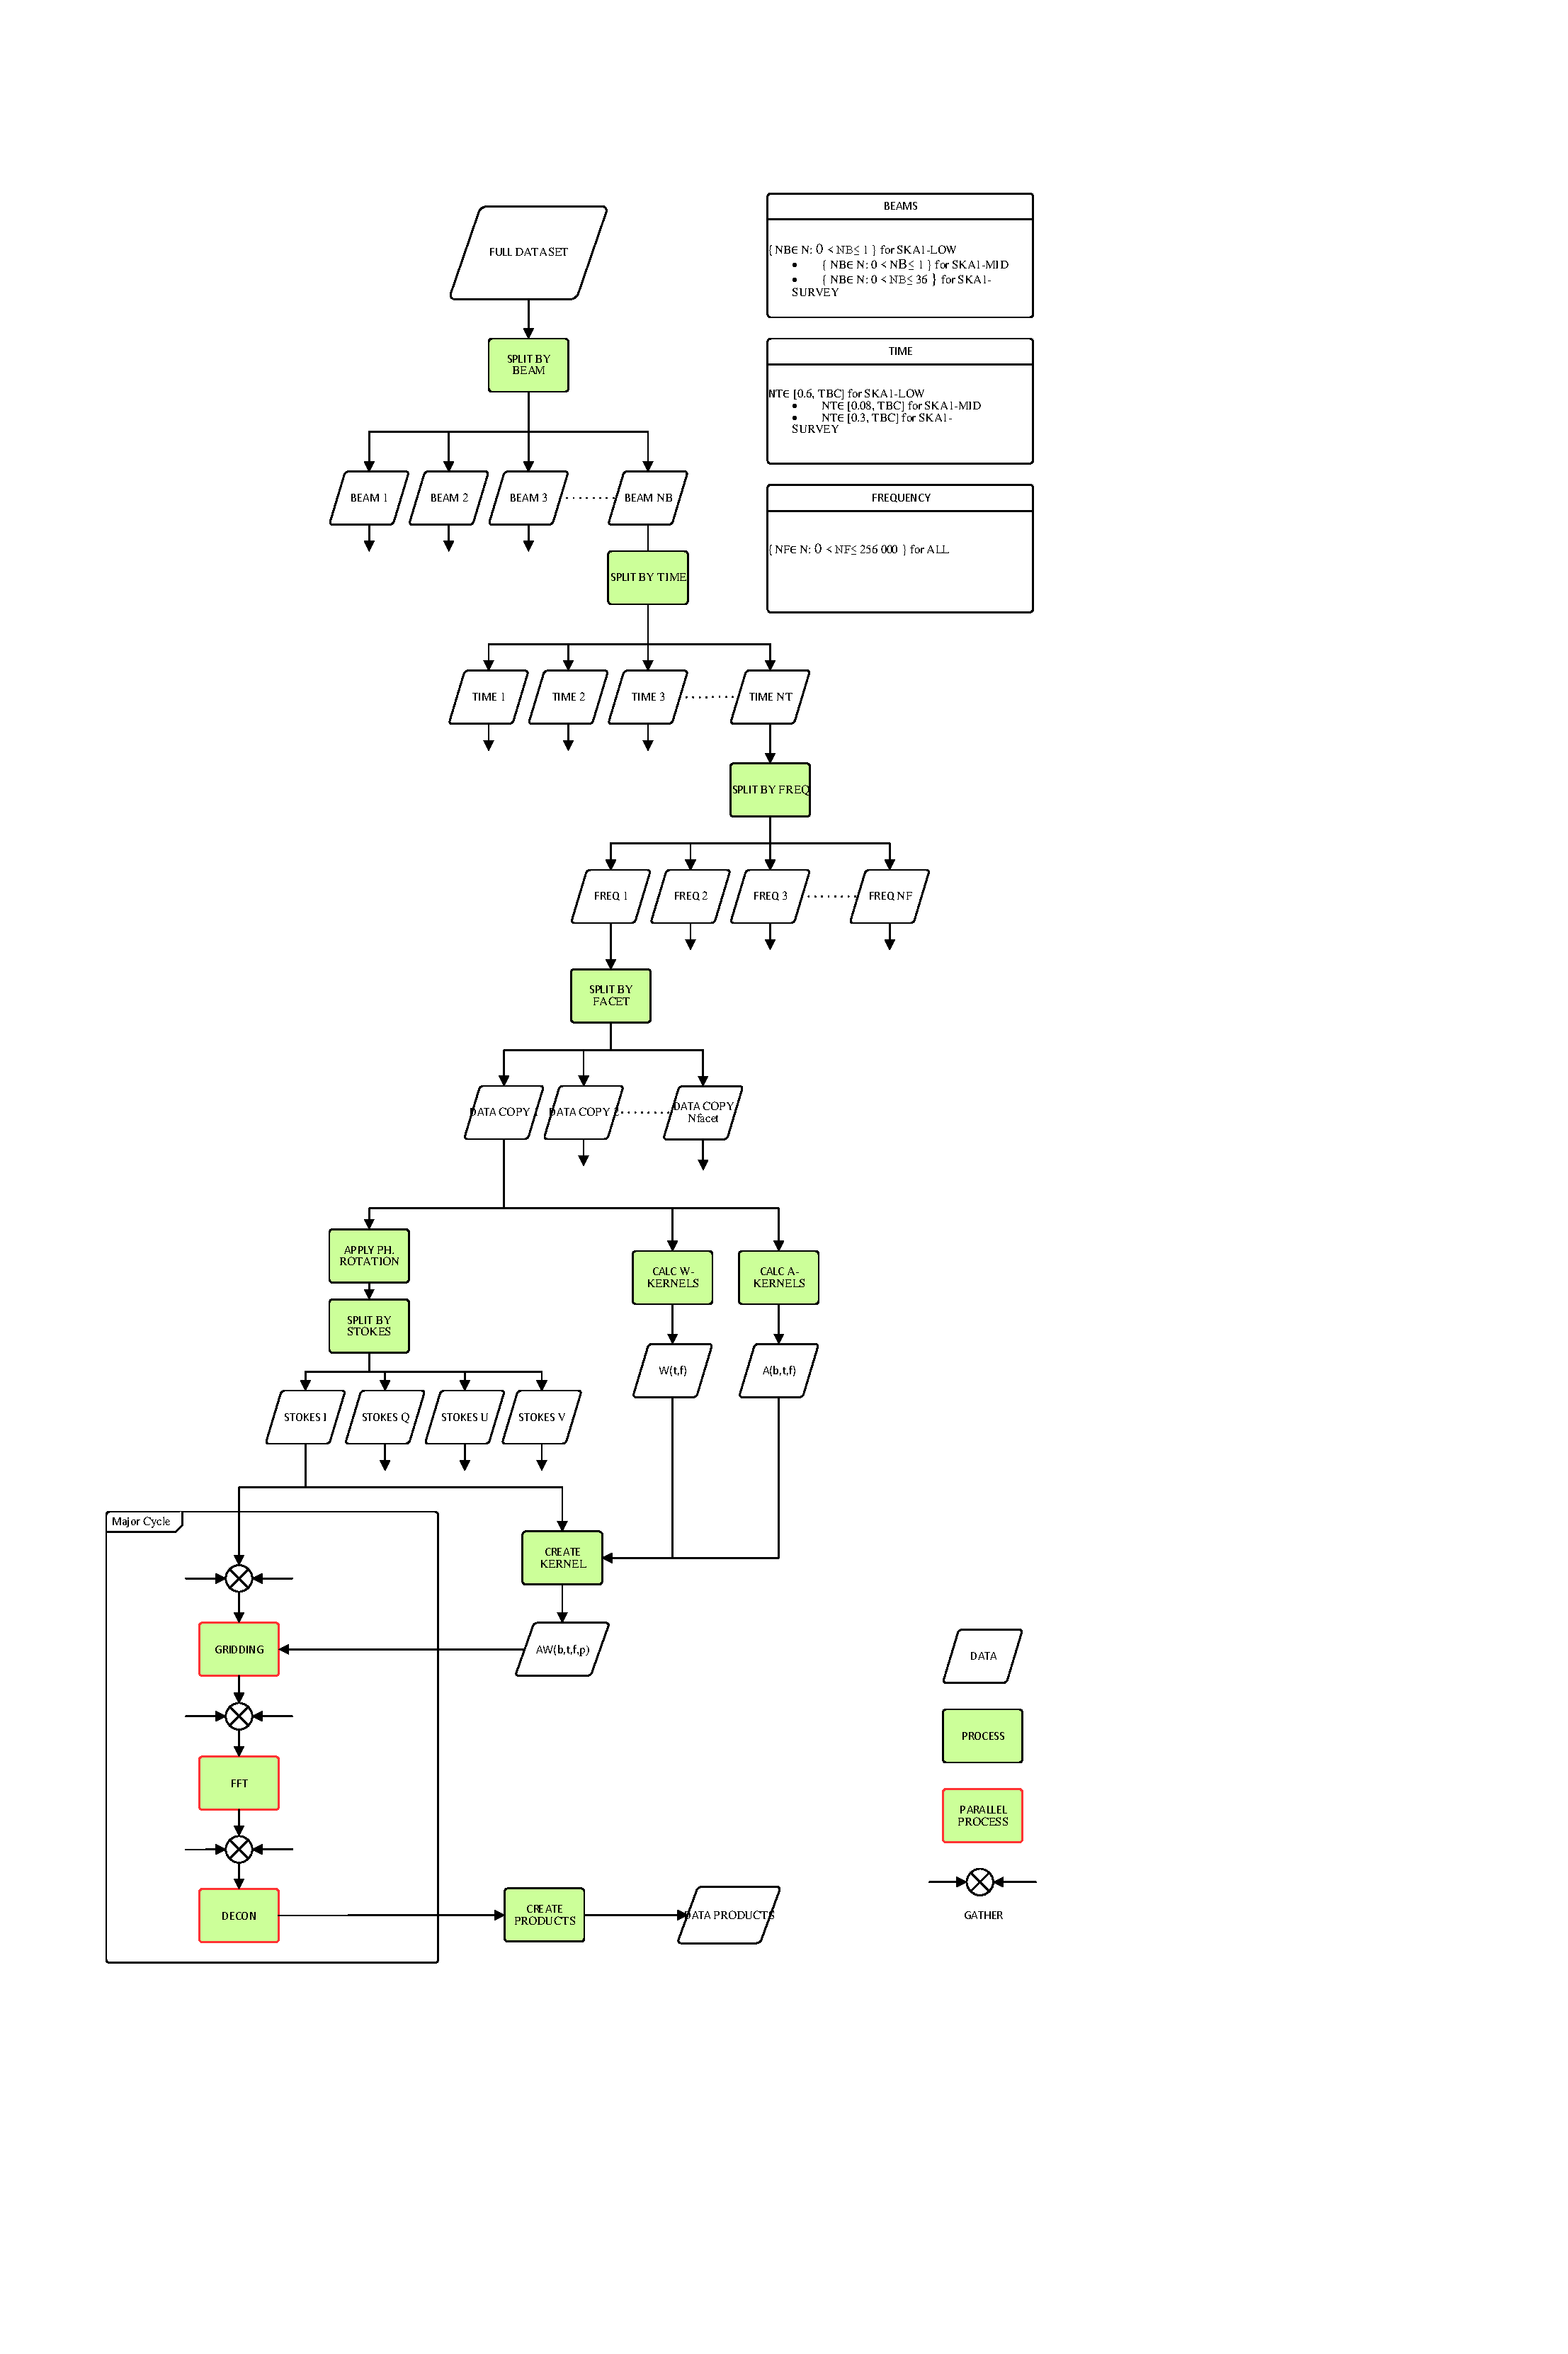
\includegraphics[width=\textwidth,trim=0 4cm 0 0]{figs/dataflow/ContinuumImagingPipeline-Overview}
  \caption{Illustration of a possible dataflow program for the
    Continuum Imaging pipeline for the SDP (calibration is not
    shown). The green rectangles are the basic computations in this
    description, i.e., the actors. Arrows represent the data
    dependencies between the actors.  See [RD02] for further
    discussion.}
  \label{fig:contdataflow}
\end{figure}



\subsection{Scheduling Blocks}

This is the full description of the processing for an observation
including the specification of the data input and outputs required
from the SDP. The details of the scheduling block will be used to
select and instantiate a dataflow program for processing of the data
during this observation.

A single dataflow program will describe \underline{all} of the
processing of data taken with single scheduling block. This is because
the same input data are used in multiple functions of the SDP (e.g.,
they may be used for real-time calibration, fast imaging, continuum
imaging and spectral imaging) and because multiple copies of the whole
input data into SDP may be very expensive. The best way of avoiding
copies and movement of data is that they are handled in a single
program.

\subsection{Granularity of the SDP program}

The diagram in Figure~\ref{fig:contdataflow} shows the possible
splitting of data that is suitable for the described algorithm.  The
splitting is done in multiple dimensions (i.e., beam, frequency, time,
facet in the above example). The granularity of the splits is an {\bf
  adjustable parameter} where:
\begin{description}
\item[upper limit] is determined by the nature of the observed data
  and algorithm: e.g., the maximum split in frequency is into the
  256000 channels
\item[lower limit] is determined by the {\bf required parallelism} to
  carry out the processing in the available time
\end{description} 

In addition to the splitting are design decisions on the granularity
of the actors used, i.e., whether they present a large sequence of
operations or individual only small routines. 

Together these decisions decide the granularity of the whole SDP
program. They will be decided by balancing following criteria:
\begin{enumerate}
\item The minimum granularity is set by the necessity to achieve the
  minimum parallelisation for the program as a whole given the
  constraints on storing the visibility data
\item Finer granularity allows for better load-balancing, potentially
  less working memory requirements, and reduces the impact of any
  failures to a smaller part of the data
\item Coarser granularity reduces message rates, reducing the
  requirement for low-latency on the interconnect
\item Coarser granularity reduces the number of actors active at any
  time, and reduces the rate at which new actors need to be fired, all
  of which should reduce overheads
\end{enumerate}

\subsection{Actors}
Actors are the processing tasks which are the individual units of
data-processing in SDP. In particular all non-trivial operations on
bulk data like visibilities and images will be carried out inside the
actors. In the example shown in Figure~\ref{fig:contdataflow} data
processing tasks like gridding, FFTs, image-plane corrections are the
actors.

A processing task operates only on the bulk data supplied to it and it
outputs results into buffer space supplied to it. It has no capability
to communicate with other processing tasks and can not request or send
bulk data. Processing tasks are referentially transparent. An example
of a processing tasks might be gridding a given set of visibilities
onto a supplied uv grid with a supplied set of convolution kernels.

The implementation scheme of tasks is not yet been decided. For
example they may be implemented either as ‘C’-API callable
sub-routines, GPU kernels, processes, services, etc. The tasks may be
single or multi-threaded internally but will present a single threaded
entry point and a single-thread of control at exit.

\section{The SDP Systems Architecture and the Dataflow System}
\label{sec:sdp-syst-arch}

In this section we show the initial mapping between dataflow concepts,
the SDP architecture, and the architecture of the primary SDP
sub-systems. The dataflow aspects of the SDP system is, like the
remainder of the system, at a preliminary design stage and therefore
detailed implementation decisions have not yet been made.

The SDP architecture adopts the dataflow programming model for the
specification of all of its primary data processing functions. 

The use of the concept of Compute Islands (see [RD03] for details)
with have very high-bandwidth communication intra-island and less so
inter-island strongly suggests that the dataflow program should be at
least partially {\bf statically scheduled}.  The static schedule will
partition the dataflow graph to Data Island level which may be as
small as small as a single compute node, or it may be composed of more
than one compute node up to the size of the compute island. This
partitioning of the graph ensure that the earliest processing stages
minimise the movement of the data between islands.

The \underline{actors} will be provided by the {\bf C.4.1} Processing
Library and {\bf C.4.4} QA components of the {\bf C.4} Pipeline
Components element. These will be referentially transparent, have
nested parallelism (most likely many-threaded parallelism), a
mechanism for caching, and access to constant data through the Local
Telescope Model. The required inputs and the produced outputs will be
declared in the interface definition of each of these components.

The \underline{channels} will be implemented in the {\bf C.3.1} Data
Manager, building on top of the {\bf C.2.2} Middleware . The channels
will be capable of buffering multiple tokens.  The tokens will be
implemented by the DataObject concept in the Data Layer.

The cluster resource allocation will be done by the {\bf C.2.5}
Scheduler subsystem in the {\bf C.2} Compute Software Platform system.

The initial \underline{static schedule} for the dataflow program will
be performed by the Data Flow Manager system in the LMC. This will
compute the static part of the schedule and configure the data flow
from the CSP to match this partitioning. The processing time estimator
will also be implemented by the Data Flow Manager.

The dataflow programs will be specified by the Data Flow Models
subsystem of the LMC.  The programming environment for the programs
and the interface declaration language for the actors will also be
implemented by the LMC.  The dataflow program for a particular
observing capability is referred to as the Logical Data Flow Graph to
reflect the fact that it has not been re-organised to be optimised for
the cluster architecture that will be used. As previously explained,
it is likely that this will not be specified as a graph, or even ever
instantiated in graph form in computer memory.

The execution engine, the dynamic scheduling engine, and the data
re-organisation engine will be implemented by the Data Manager
subsystem from the Data Layer. The required capabilities of the
dynamic scheduling engine and the data-re-organisation engine will be
specified once the design of the compute platform is more precisely
known and an initial analysis of data re-organisation has been
performed.

%  Add the bibliography
\clearpage
\addcontentsline{toc}{section}{References}
\bibliography{skasdp}%


\end{document}

%%% Local Variables: 
%%% mode: latex
%%% TeX-master: t
%%% End: 
